\documentclass{pgnotes}

\title{Fire}

\begin{document}

\maketitle

\section{Fire Triangle}
\label{sec:fire-triangle}

The fire triangle shows three required components:

\begin{figure}[htbp]
  \centering
  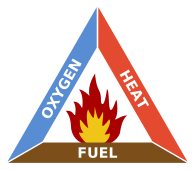
\includegraphics[width=0.5\linewidth]{fire_triangle}
  \caption{Fire triangle}
  \label{fig:fire-triangle}
\end{figure}

\begin{description}
\item[Fuel]
to burn.
\item[Heat]
to start the fire.
\item[Oxygen]
to sustain the fire.
\end{description}

\section{Consequences of fire}
\label{sec:consequences-of-fire}

\begin{itemize}
\item
  Destruction of the data centre / server room itself.
\item
  Destruction of the harware inside the data centre / server room.
\item
  Loss of data caused by the destruction of data centre equipment.
\item
  Interruption to business continuity due to unavailablility of the data
  centre during or after a fire event.
\end{itemize}

\section{Data centre-specific factors}
\label{sec:data-centre-specific-factors}

\begin{enumerate}
\item
  Data centres are not normally occupied in the normal course of work.
  In fact, a properly run data centre should rarely need humans inside
  it for extended periods. However, this means that fires are less
  likely to be noticed.
\item
  Smaller server closets are particularly at risk of being used as
  unofficial storage areas for equipment, paperwork and indeed rubbish.
  Any solid object is potential fuel for a fire and shouldn't be there.
\item
  Data centres run at elevated temperatures to conserve electrical
  power. While an office might be at 21C, a server room may be at 25C.
\item
  Elevated temperatures lead to lower relative humidity. Less dampness
  makes it easier for a fire to progress, and can worsen the effects of
  electrical sparks.
\item
  A large amount of electrical equipment is present in a relatively
  small area.
\item
  UPS systems include batteries. Lead-acid cells can vent hydrogen if
  overcharged, and lithium-ion batteries can easily catch fire.
\end{enumerate}

\section{Actions required}
\label{sec:actions-required}

\begin{description}
\item[Prevention]
of fire outbreak.
\item[Mitigation]
of effects a potential fire can have.
\item[Detection]
of a fire at the earliest possible stage.
\item[Alerting]
persons inside and responsible persons outside the data center
environment that a fire has started.
\item[Suppression]
of the fire.
\end{description}

\section{Fire classes}
\label{sec:fire-classes}

Fires can be categorised into a number of classes depending on the type
of fire, . Knowing the class of a fire helps when choosing how to fight
it.

\autoimage{fire_classes}{Fire classes}{fire-classes}

\subsection{Prevention strategies}
\label{sec:prevention-strategies}

The easiest prevention strategies involve reducing the availability of
fuel, heat and oxygen.

\subsubsection{Fuel}
\label{sec:fuel}

The easiest way to reduce the risk of fire in a data centre is to reduce
the amount of fuel:

\begin{itemize}
\item
  All equipment should be either racked or wall mounted if relevant.
  Nothing should be allowed on the floor.
\item
  Decomissioned or unused equipment should be removed.
\item
  Wiring that is obsolete and unlikely to ever be reused should be fully
  removed.
\item
  The data centre must not be used as a storage area, either for
  equipment nor paperwork.
\item
  If a small working desk is provided inside the data centre, it must be
  for occasional use while performing a task and a ``clean desk'' policy
  must be in place.
\item
  Rubbish (e.g.~packing boxes) must be removed immediately from the data
  centre after any work is done. If packaging is not going to be
  immediately disposed of, it should be stored elsewhere outside the
  data centre.
\item
  The data centre must be kept clean and free of dust.
\item
  Manufacturer's instructions regarding batteries in particular must be
  fully complied with.
\end{itemize}

\subsection{Heat}
\label{sec:heat}

In a closed volume of air, raising the temperature (as would be the case
in a data centre) has two effects:

\begin{itemize}
\item
  Fires are easier to sustain.
\item
  Reduced humidity, causing increased risk of sparks.
\end{itemize}

\subsection{Oxygen}
\label{sec:oxygen}

Oxygen is present at approximately in the air under normal conditions:

\begin{itemize}
\item
  Normally this is just a physical fact that has to be lived with!
\item
  A very small number of data centres worldwide are equipped with a
  hypoxic air supply system which reduces the oxygen concentration to
  approximately . Fires cannot start or be sustained under these
  conditions.
\item
  Although hypoxic air systems are not commonly deployed, reducing the
  oxygen content is a key part of gaseous fire suppression systems,
  which function differently.
\end{itemize}

\section{Mitigation strategies}
\label{sec:mitigation-strategies}

Sometimes, fire will damage or destroy the data centre, or the building
in which it is situated.

\begin{itemize}
\item
  Just as we have redundancy levels in power and cooling, consider
  having a secondary data centre location. This will involve duplication
  of hardware, mirroring of data and configuration, and may involve
  complex network routing.
\item
  Virtualisation can make it easier to migrate many workloads from one
  location to another.
\end{itemize}

\section{Detection methods}
\label{sec:detection-methods}

Fire is detected normally by its byproducts: smoke and heat.

\begin{description}
\item[Smoke detectors]
signal an alarm when they detect smoke particles in the air. Two
methods:

\begin{description}
\item[Ionisation]
detectors use radio isotopes to ionise the air, allowing it to conduct
electric current. When a change is detected due to the presence of
smoke, an alarm is triggered.
\item[Photoelectric]
detectors use a light source passed through the air that is incident on
a photoelectric cell. When the light becomes sufficiently obscured by
smoke, an alarm is triggered.
\end{description}
\item[Heat detectors]
signal an alarm based on temperature:

\begin{description}
\item[Fixed temperature]
detectors activate when the ambient temperature exceeds the threshold
temperature.
\item[Rate-of-rise]
temperature detectors activate when a the rise in temperature in a fixed
period of time exceeds the maximum allowed.
\end{description}
\end{description}

\subsection{Detector types}
\label{sec:detector-types}

\begin{description}
\item[Area]
detectors are what we are familiar with from non-data centre
environments. A detection head is placed in the overall area.

\begin{itemize}
\item
  Air conditioning system will dilute the air sufficiently that large
  quantities of smoke will be required before an alarm is raised.
\end{itemize}
\item[Aspirating]
smoke detectors (ASDs) uses a fan to suck air from a sampling pipe with
one or more sampling heads into a detection chamber.
\end{description}

\subsection{Fire panel}
\label{sec:fire-panel}

A local fire panel is often provided in a data centre. Its main
functions are:

\begin{itemize}
\item
  Receive inputs from detection devices.
\item
  Alerting the presence of fire inside and outside the data centre
  using: audible warning devices (bell, syren, klaxon), visual warning
  devices (strobe), signalling staff and BMS.
\item
  Activating fire suppression systems, HVAC shutdown, power shutdown.
\item
  If the data centre is part of a larger facility, the data centre's
  fire alarm/alerting/suppression system will need to be interlocked
  correctly with the main system.
\item
  Allowing remote visibility through the use of a remote annunciator,
  repeater or slave panel (same meaning for all!).
\end{itemize}

\section{Extinguishants}
\label{sec:extinguishants}

Extinguishants are broadly divided into gaseous, removing oxygen and
water, removing heat.

\end{document}

